\newpage
\section{Entwurf}
Dieses Kapitel befasst sich mit der Struktur der Implementierung. Damit wird die Herangehensweise beschrieben und es wird erläutert, wieso bestimmte Entscheidungen getroffen wurden.

\subsection{Hardware}
Um die Hardwarekosten bei einer Skalierung für die Positionsbestimmung niedrig zu halten, wurde der \microphone \platz auf dem Master-Knoten verbaut und dementsprechend die Lautsprecher auf dem Slave-Knoten. Diese Variante hat allerdings den Nachteil, dass nur ein Slave abgefragt werden kann. Somit braucht es bei drei Slaves mindestens drei Schallmessungen gegenüber einer Messung. Die verwendete Variante hat jedoch den Vorteil, dass der Master entscheidet, mit welchem Slave eine Messung vorgenommen wird. Weiterhin ist der Softwareaufwand für eine Wiederholung der Messung aufgrund von Fehlern geringer.

\subsection{Struktur}
Zuerst wird der \microphone \platz dahingehend untersucht, ob er überhaupt schnell genug für die Positionsbestimmung ist. Danach wird ein Versuchsaufbau nach dem folgenden Blockschaltbild \ref{img:kommunikation_module} eingerichtet. Das Blockschaltbild teilt den Versuchsaufbau in verschiedene Module auf -- damit lassen sich Abweichungen besser zuordnen.

\begin{figure}[H]
\centering
\hspace*{-2.6cm}
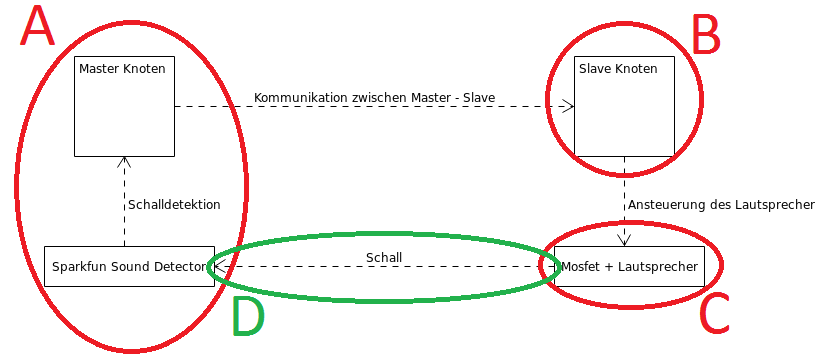
\includegraphics[width=1.3\textwidth]{images/Kommunikation_Module.png}
\caption{Versuchsaufbau, unterteilt in Module}
\label{img:kommunikation_module}
\end{figure}

%newpage einfügen

Nachdem die einzelnen Module getestet worden sind, wird der Aufruf der RIOT Funktion $getSystemTime()$ geprüft. Die Prüfung dieser Funktion ist wichtig, weil sie die aktuelle Systemzeit ausliest. Sobald der Ton das Mikrofon passiert, wird diese Funktion aufgerufen. Im Rahmen des Funktionsaufrufes entsteht eine zeitliche Abweichung mit einer hohen Relevanz, da mehrere CPU-Zyklen benötigt werden, bevor die Systemzeit in der Variable gespeichert wird. Anschließend wird die Zeitsynchronisation überprüft. Danach folgt ein Versuch, bei dem anstatt der Funkkommunikation vom \board, das \funkempfaenger \platz Modul verwendet wird. Die verwendete Software für die einzelnen Module ist auf dem mitgelieferten USB-Stick gespeichert. Bei den jeweiligen Modulen ist der \si{GATE}-Pin bei dem Master an dem Pin \si{PB23} angeschlossen. Für den Slave wird immer Pin \si{PA18} verwendet. Abbildungen \ref{img:verdrahtungsplan_master} und \ref{img:verdrahtungsplan_slave} zeigen die Verdrahtungen.

\begin{figure}[H]
	\centering
	\hspace*{-2cm}
	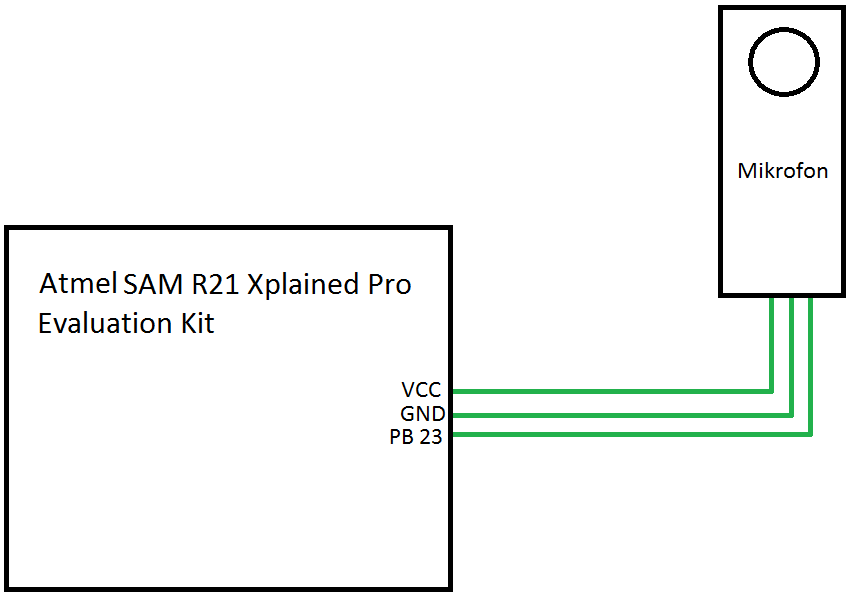
\includegraphics[width=0.6\textwidth]{images/schaltplan_master.png}
	\caption{Verdrahtungsplan Master}
	\label{img:verdrahtungsplan_master}
\end{figure}

\begin{figure}[H]
	\centering
	\hspace*{-2cm}
	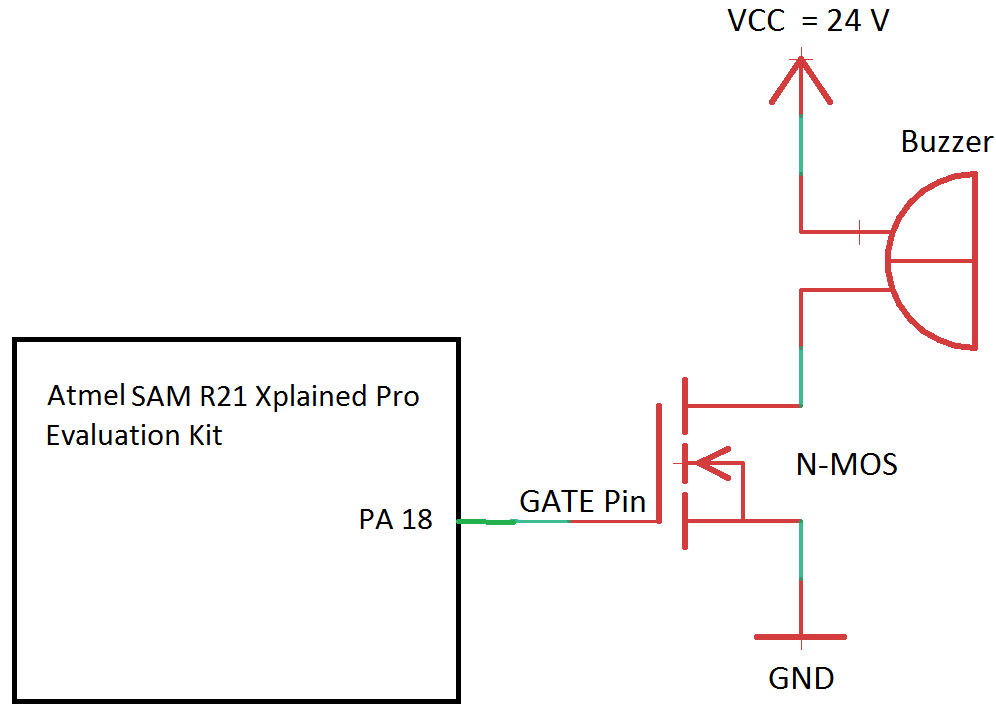
\includegraphics[width=0.6\textwidth]{images/schaltplan_slave.png}
	\caption{Verdrahtungsplan Slave}
	\label{img:verdrahtungsplan_slave}
\end{figure}




